\section{Operads using coends.}\label{sec:opd}
Since they were introduced by P\@. May in his \cite{may1972geometry} to solve a problem in algebraic topology,\footnote{There are several reasons why algebraic topologists are interested in spaces $Y$ which are homotopy equivalent to $\Omega X$; they are much more interested in spaces $Y\simeq \Omega^n X$, and in spaces such that ``$Y\simeq \Omega^\infty X$'': these are called \emph{infinite loop spaces}. \cite{may1972geometry} offers a way to recognize infinite loop spaces among all spaces. See \cite{adams1978infinite} for more informations.} it has been clear that operads are monoid-like objects in some category of functors; making this analogy a precise statement, using the power of coend-fu, is the content of Kelly's \cite{Kelly2005a}, which we follow here almost \emph{verbatim}.

A certain acquaintance with the machinery of operads is a fundamental prerequisite to follow the discussion; unfortunately, given the plethora of different interpretation of the theory, and different areas of mathematics where the notion of operad arises, the beginners (the author of the present note is undoubtedly among them) may feel rather disoriented when approaching any book on the subject, so it's extremely difficult to advise a single, comprehensive reference. 

Among classical textbooks, we can't help but mention the founder \cite{may1972geometry}, as well as more recent monographies like \cite{loday2012algebraic, markl2007operads} written respectively from the algebraist's and topologist's point of view. Among less classical and yet extremely valid points of view, the author profited a lot from a lucid, and unfortunately still unfinished, online draft \cite{trimblerads} written by T\@. Trimble.

\paragraph{\bf Local conventions.} Along the whole section we will adopt the following notation and conventions:
\begin{itemize}
\item $\P$ is the \emph{groupoid of natural numbers}, \ie the category having objects the nonempty sets $\{1,\dots, n\}$ (denoted as $n$ for short, assuming that $0 = \varnothing$) where $\P(m,n)=\varnothing$ if $n\neq m$ and $S_n$ (the group of bijections of $n$-element sets) if $n=m$. It is evident that $\P$ is the disjoint union of groups $\coprod_{n\ge 0} S_n$ in the category $\Gpd$ of groupoids.
\item $\V$ is a fixed \emph{B\'enabou cosmos} (\ie a bicomplete closed symmetric monoidal category, ``a good setting to do enriched category theory'', see Notation \refbf{cosmo}).
\end{itemize}
Notice that $\P$ has a symmetric monoidal structure, with tensor the \emph{sum} of natural numbers; the action on arrows is given by $(\sigma,\tau)\mapsto \sigma+\tau$ defined acting as $\sigma$ on the set $\{1,\dots, m\}$ and as $\tau$ on the set $\{m+1,\dots, m+n\}$ (these permutations are called \emph{shuffles}).
\subsection{Convolution product} We begin our discussion presenting a general theorem on monoidal categories, first outlined by B\@. Day: it will be utterly generalized in our Appendix \refbf{sec:promono}.

The rough idea is the following: in the same way the set of regular functions $f \colon G \to \mathbb{C}$ on a topological group $G$ acquires a \emph{convolution} product given by $(f,g)(x) = \int_G f(xy^{-1})g(y)dy$ (the integral sign here is not an end!), we can endow the \emph{category of co/presheaves} $F\colon \C\to\V$ with a monoidal structure induced by a monoidal structure on $\C$, which is different from the pointwise one, induced by the monoidality of the codomain. This is called the \emph{convolution product} of functors; appendix \textbf{A} will give a generalization of this point of view in form of exercises (see in particular Exercises \refbf{ex1}, \refbf{ex2}).
\begin{definition}[Day convolution]\label{day} If $\C$ is a symmetric monoidal category, then the functor category $[\C,\V]$ is itself a B\'enabou cosmos with respect to the monoidal structure given by \emph{Day convolution product}: given $F,G\in[\C,\V]$ we define
\[
F\ast G := \int^{cd}\C(c\otimes d,\firstblank)\cdot Fc\otimes Gd
\] 
where we recall that $X\cdot V$ for $X\in\Sets,V\in \V$ is the \emph{copower} (or \emph{tensor}) $X\cdot V$ such that
\[
\V(X\cdot V,W)\cong \Sets(X, \V(V,W)).
\]
\end{definition}
\begin{notat}
In the following sections we will make use of the ``Einstein notation'' for co/ends defined in \refbf{einstein}; this will compactify a lot the exposition. A fundamental rule to avoid getting lost is the following, really akin to the Einstein convention for tensor operations: variables of integration are paired as subscript\hyp{}superscript, and whenever they are paired a co/end operation is implicit.

Without smart ideas to specify the difference we are forced to maintain all integral signs, to discern ends from coends. In Einstein notation we write the convolution as
\[
F\ast G = \int^{cd} \C^{c\otimes d}_{(\firstblank)} F_c G_d
\]
\end{notat}
\begin{proof}
We have to show that this really defines a monoidal structure:
\begin{itemize}
\item Associativity follows from the associativity of the tensor product on $\C$ and the ninja Yoneda lemma (see the remark above for the Einstein convention; it is also harmless to suppress the distinction between monoidal products in $\V$ and $\Sets$-tensors, since the distinction can be easily devised with a ``dimensionality check''):
\begin{align*}
[F\ast(G\ast H)]_x &= \int^{ab}\C^{a\otimes b}_x F_a (G\ast H)_b\\
&\cong \int^{ab}\C^{a\otimes b}_x \int^{cd}\C^{c\otimes d}_b F_a G_c H_d\\
&\cong \int^{abcd}\C^{a\otimes b}_x \C^{c\otimes d}_b F_a G_c H_d\\
&\cong \int^{acd}\C^{a\otimes(c\otimes d)}_x F_a G_c H_d\\
[(F\ast G)\ast H]_x&\cong \int^{acd}\C^{(a\otimes c)\otimes d}_x F_a G_c H_d.
\end{align*}
\item (Right) unitality : choose $J=\yon_I=\C(I,\firstblank)$ and notice that the ninja Yoneda lemma implies that
\begin{align*}
[F\ast J]_x&\cong \int^{cd}\C^{c\otimes d}_x F_c J_d\\
&\cong \int^{cd}\C^{c\otimes d}_x \C^I_d F_c\\
&\cong \int^c\C^{c\otimes I}_x F_c\cong F_x.
\end{align*}
\item Left unitality is totally analogous.
\end{itemize}
\begin{example}[Subdivision and joins as convolutions]
Compare Example \refbf{ex.sub} and the definition of \emph{join} of \emph{augmented}\footnote{The category $\bDelta$ lacks an initial object $[-1] = \varnothing$; if we add this colimit we get a category $\bDelta_+$, and an \emph{augmented} simplicial set is a presheaf on $\bDelta_+$; the category of augmented simplicial sets is denoted $\sSet_+$. There is a triple of adjoints induced by the inclusion $i\colon \bDelta \subset \bDelta_+$ and linking the categories of simplicial and augmented simplicial sets. The join operation is easily seen to restrict to simplicial sets (identified with augmented simplicial sets with empty set of $(-1)$-simplices) giving a monoidal structure on $\sSet$.} simplicial sets given in \cite{Joy}: given $X, Y \in\sSet_+$ we define
\[
X \star Y = \int^{p,q} X_p \times Y_q \times \bDelta(\firstblank, p\oplus q)
\]
where $\oplus$ is the \emph{ordinal sum} operation (see again \cite{Joy} or rather our \refbf{ex.sub}).
\end{example}
The category $[\C,\V]$ is left and right closed with respect to this monoidal structure: the exponential $G/H$ (or rather the functor $G/\firstblank$ which is right adjoint to $\firstblank\ast G$) is given by
\[
G/H := \int_c [Gc,H(c\otimes \firstblank)]
\]
where $[\firstblank,\secondblank]$ is the internal hom in $\V$, and often denoted $\llbracket G,H\rrbracket$. We can compute directly that
\begin{align*}
 \Nat(F\ast G,H) &\cong \int_c\V\big((F\ast G)c,Hc\big) \\
 &\cong \int_c {\V}\left(  \int^{ab}\C^{a\otimes b}_c F_a G_b,\;H_c \right)\\
&\cong  \int_{abc}{\V}\big( \C^{a\otimes b}_c F_a G_b,\;H_c \big) \\
&\cong  \int_{abc} {\V} \big(F_a, [\C^{a\otimes b}_c G_b,H_c]\big)\\
&\cong  \int_{abc} {\V} \big(F_a, \big[G_b,[\C^{a\otimes b}_c,H_c]\big]\big) \\
&\cong  \int_{ab} {\V} \big(F_a,  \big[G_b, \int_c [\C^{a\otimes b}_c,H_c]\big]\big)\\
&\cong \int_{ab} {\V} \big(F_a,[G_b,H_{a\otimes b}]\big) \\
&\cong \int_a {\V}\left(F_a, \int_b[G_b,H_{a\otimes b}]\right)\\
&\cong  \int_a {\V}(F_a,\llbracket G,H\rrbracket_a)\\
&\cong \Nat\big(F,\llbracket G,H\rrbracket\big).\qedhere
\end{align*}
\end{proof}
\begin{remark}
In the particular case $\C=\P$ this means that $[\P,\V]$ is monoidal closed if we define
\begin{align*}
\displaystyle (F\ast G)_k &:= \int^{mn}\P(m+n,k)\cdot F_m \otimes G_n\\
\displaystyle \llbracket F,G\rrbracket_k &:= \int_n [F_n, G_{n+k}]
\end{align*}
In particular, we have the formula
\[
F_1\ast\dots\ast F_n = \int^{k_1,\dots, k_n} \P\Big(\sum k_i,\firstblank\Big)\cdot F_1 k_1 \otimes \dots \otimes F_nk_n.
\]
for the iterated convolution of $F_1,\dots, F_n\in [\C, \V]$, which will become useful in a while.
\end{remark}
The gist of the definition of a $\V$-operad lies in an additional monoidal structure on $[\P,\V]$, defined by means of the Day convolution:
\begin{definition}[Diamond product on \protect{$[\P,\V]$}]
Let $F,G\in [\P,\V]$. Define
\[
F\diamond G:=\int^m Fm\otimes G^{\ast m},
\]
where $G^{\ast m} := G\ast\dots \ast G$.
\end{definition}
Associativity exploits the following
\begin{lemma}
 There exists a natural equivalence $(F\diamond G)^{\ast m}\cong F^{\ast m}\diamond G$.
\end{lemma} 
\begin{proof}
It's a formal manipulation:
\begin{align*}
 (F\diamond G)^{\ast m}&=\int^{\vec n_i} \P\Big(\sum n_i,\firstblank\Big)\cdot (F\diamond G)n_1\otimes\dots\otimes (F\diamond G)n_m \\
&\cong \int^{\vec n_i,k_i}\P\Big(\sum n_i,\firstblank\Big)\cdot Fk_1\otimes G^{\ast k_1}n_1\otimes\dots\otimes Fk_m\otimes G^{\ast k_m}n_m\\
&\cong \int^{\vec n_i,\vec k_i}Fk_1\otimes\dots\otimes Fk_m\otimes \P\Big(\sum n_i,\firstblank\Big)\cdot G^{\ast k_1}n_1\otimes\dots G^{\ast k_m}n_m\\
&\cong \int^{\vec k_i} Fk_1\otimes\dots\otimes Fk_m\otimes \big(G^{\ast k_1}\ast \dots\ast G^{\ast k_m}\big)\\
&\cong \int^{\vec k_i} Fk_1\otimes\dots\otimes Fk_m\otimes G^{\ast \sum k_i}\\
\textsc{ninja} &\cong \int^{\vec k_i,r}\P\Big(\sum k_i,r\Big)\otimes Fk_1\otimes\dots\otimes Fk_m\otimes G^{\ast r}\\
&\cong \int^r F^{\ast m}r\ast Gr = F^{\ast m}\diamond G
\end{align*}
(we used a compact notation for $\int^{\vec n_i}=\int^{n_1,\dots,n_m}$; the ninja Yoneda Lemma is used in the form $\displaystyle G^{\ast n}\cong \int^r\P(n,t)\cdot Gt = \P(n,\firstblank)\diamond G$, because $(n,G)\mapsto G^{\ast n}$ is a bifunctor $\P \times [\P, \V]\to [\P, \V]$).
\end{proof}
Associativity of the diamond product now follows at once: we have
\begin{align*}
 (F\diamond(G\diamond H))(k) & =\int^m Fm\otimes (G\diamond H)^{\ast m}k\\
&\cong \int^m Fm\otimes (G^{\ast m}\diamond H)k\\
&\cong \int^{m,l}Fm\otimes G^{\ast m}l\otimes H^{\ast l}k\\
&\cong \int^l (F\diamond G)l\otimes H^{\ast l}k\\
& = ((F\diamond G)\diamond H)(k).
\end{align*}
A unit object for the $\diamond$-product is $J=\P(1,\firstblank)\cdot I$; indeed $J(1)=I$, $J(n)=\varnothing_\V$ for any $n\neq 1$ and the ninja Yoneda lemma applies on both sides to show unitality rules:
\begin{itemize}
 \item On the left one has 
\[
J\diamond F = \int^m Jm\otimes F^{\ast m}=\int^m \P(1,m)\cdot F^{\ast m} \cong F^{\ast 1}=F.
\]
\item On the right, $G\diamond J\cong G$ once noticed that $J^{\ast m}\cong \P(m,\firstblank)\cdot I$ since
\begin{align*}
 J^{\ast m} & = \int^{\vec n_i}\P\Big(\sum n_i,\firstblank\Big)\cdot \P(1,n_1)\cdot\dots\cdot \P(1,n_m)\cdot I\\
\textsc{ninja} &\cong \P(1+\dots+1,\firstblank)\cdot I = \P(m,\firstblank)\cdot I 
\end{align*}
because 
\[\int^{\vec n_i}\P(n_1+\dots+n_m,\firstblank)\cdot \P(1,n_i)\cong \P(n_1+\dots+n_{i-1}+1+n_{i+1}+\dots + n_m,\firstblank),\]
for any $1\le i\le m$ (it is again an instance of the ninja Yoneda Lemma). One has
\[
 G\diamond J = \int^m Gm\otimes J^{\ast m}\cong \int^m Gm\otimes \P(m,\firstblank)\cdot I\cong G.
\]
\end{itemize}
\begin{theorem}
 The $\diamond$-monoidal structure is left closed, but not right closed.
\end{theorem}
\begin{proof}
It is a formal manipulation:
\begin{align*}
\Nat(F\diamond G,H)&\cong \Nat\Big( \int^m Fm\otimes G^{\ast m}, H \Big)\\
&\cong \int_k \V\Big( \int^m Fm\otimes G^{\ast m}, H \Big)\\
&\cong \int_{km}\V(Fm, [G^{\ast m}k,Hk])\\
&\cong \int_m \V(Fm, \int_k[G^{\ast m}k,Hk])
\end{align*}
which is equal to $\Nat(F,\{G,H\})$ if we define $\{G,H\}m=\displaystyle \int_k[G^{\ast m}k,Hk]$. Hence the functor $(\firstblank)\diamond G$ has a right adjoint for any $G$. 

The functor $F\diamond (\firstblank)$ can't have such an adjoint (Incidentally, this shows also that the diamond product can't come from a convolution product with respect to a \emph{promonoidal structure} in the sense of Proposition \refbf{promonoshit}. Re-read this result after having gone through Appendix \textbf{A}!). We leave the reader think about the reason.
\end{proof}
\begin{definition}
An \emph{operad} in $\V$ consists of a monoid object in $[\P,\V]$ endowed with the $(\diamond,\{\firstblank,\secondblank\})$ left-closed monoidal structure.

More explicitly, an operad is a functor $T\in [\P,\V]$ endowed with a natural transformation called \emph{multiplication}, $\mu\colon T\diamond T\to T$ and a \emph{unit} $\eta\colon J\to T$ such that
\begin{center} 
 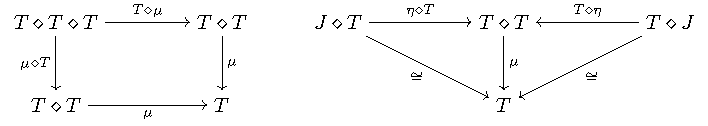
\includegraphics[scale=1]{figures/fig23} 
 \end{center}
are commutative diagrams. 
\end{definition}
%
\begin{definition}[Endomorphism operad]
For any $F\in [\P,\V]$ the object $\{F,F\}$ is an operad whose multiplication is the adjunct of the arrow
\begin{center} 
 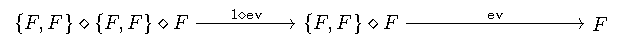
\includegraphics[scale=1]{figures/fig24} 
 \end{center}
and whose unit is the adjunct of the isomorphism $J\diamond F\cong F$.
\end{definition}
Unraveling the previous definition, we can notice that an operad in $\V$ consists of
\begin{itemize}
\item Giving a natural transformation $\eta\colon J\to T$ amounts to a map $\eta_1\colon I\to T(1)$, since $J(1)=I, J(n)=\varnothing$ for $n\neq 1$;
\item Giving a natural transformation $\mu\colon T\diamond T\to T$, in view of the universal property of the two coends involved, amounts to give a cowedge
\begin{center} 
 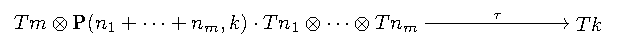
\includegraphics[scale=1]{figures/fig25} 
 \end{center}
for any $m,n_1,\dots, n_m,k\in\N$, natural in $k$ and the $n_i$ and such that the following diagram commutes:
\begin{center} 
 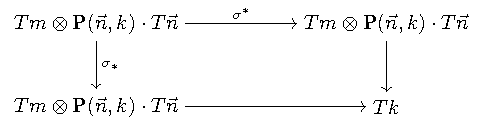
\includegraphics[scale=1]{figures/fig26} 
 \end{center}
(the notation is self-evident) for every morphism $\sigma\in \P$. This is equivalent to a transformation
\begin{center} 
 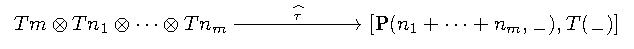
\includegraphics[scale=1]{figures/fig27} 
 \end{center}
(considering the $n_i$ fixed and the first functor constant in $k$) \ie, by the Yoneda Lemma a natural transformation
\begin{center} 
 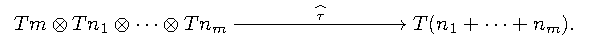
\includegraphics[scale=1]{figures/fig28} 
 \end{center}
\end{itemize}
This concludes the discussion, as it is precisely the definition of operad given in \cite{MR1436914}. It only remains to verify that all the axioms given there are satisfied. This is a tedious but necessary exercise.
% \subsection{Generalizations of operads}
% \todo[inline]{generalized operads (con $G(n)$)}
% \todo[inline]{gambo-joy}
% \todo[inline]{zawadowski}
% \todo[inline]{trimble}
\begin{exerciseset}
\begin{exercisepoints}
\item Show that the convolution product on $[\C, \V]$ results as the following left Kan extension:
\[
\xymatrix{
	\C \times \C \ar[d]_\odot \ar[r]^{F\times G} & \V \times \V \ar[r]^(.6){\otimes_\V} & \V \\
	\C \ar@{.>}@/_1pc/[urr]
}
\]
\item Define two functors
\begin{gather*}
\Phi\colon [\P,\V]\to \V \qquad \text{(evaluation at $0$)}\\
\Psi\colon \V \to [\P,\V]\qquad \text{(the left adjoint to } \Phi)
\end{gather*}
Prove that $\Psi(a\otimes b)\cong \Psi a\otimes \Psi b$ and $\Phi\circ\Psi\cong 1$; finally, if $a\in \V$ is identified with the constant functor in $a$, then $[\P,\V](a\ast F,G)\cong \V(a,[F,G])$, where
\[
[F,G] := \int_n \V(Fn, Gn).
\]
\end{exercisepoints}
\end{exerciseset}